\FILE{specifying-workflows.tex}

\section{Specifying Workflows}\label{specifying-workflows}

The workflow definition for cloudmesh is rather simple and intuitive.
An example is provided in Figure~\ref{fig:workflow-example}.  Here a
DAG with three nodes ar specified ($start \rightarrow fetch-data \rightarrow
compute \rightarrow analyze \rightarrow end $). The workflow executes three
scripts (test-[fetch-data,compute,analyze].sh). It contains a specific start and end noode.

\subsection{Dependencies}

Each dependency is specified in the {\em dependency} section while
providing sequences of names in a list such as
\verb|-start,fetch-data| or in our case where 3 more nodes are defined an
additional node is appended with \verb|,compute,analyze,end|.

In case one wants to execute nodes in parallel we can simply define
them through a list such as 

\begin{minted}[breaklines]{yaml}
  dependencies:
    - start,a,end
    - start,b,end
    - start,c,end
\end{minted}

if the names of the nodes were $a$, $b$, and $c$. 


\subsection{Nodes}

Nodes can be customized in various ways within the workflow
configuration YAML file, including their job types (python, sh, jupyter,
or slurm), their virtual Python environment (by specifying
\texttt{venv}), their appearance on the graph, and other
characteristics.  This is controoled throgh a number of attributes
used by the nodes in the DAG The attributes summarized in
Table~\ref{tab:node-attributes}.

\begin{figure}
\begin{minted}[breaklines]{yaml}
workflow:
  nodes:
    start:
       name: start
    fetch-data:
       name: fetch-data
       user: gregor
       host: localhost
       kind: local
       status: ready
       label: '{name}\nprogress={progress}'
       script: test-fetch-data.sh
    compute:
       name: compute
       user: gregor
       host: localhost
       kind: local
       status: ready
       label: '{name}\nprogress={progress}'
       script: test-compute.sh
    analyze:
      name: analyze
      user: gregor
      host: localhost
      kind: local
      status: ready
      label: '{name}\nprogress={progress}'
      script: test-analyze.sh
    end:
       name: end
  dependencies:
    - sart,fetch-data,compute,anlayze,end
\end{minted}
\caption{Workflow YAML Configuration file}\label{fig:workflow-example}
\label{fig:yaml-file}
\end{figure}

\begin{table}[htb]
\caption{Node attributes}\label{tab:node-attributes}
\resizebox{1.0\columnwidth}{!}{
\begin{tabular}{|l|p{6cm}|}
\hline
{\bf Attribute} & {\bf Description} \\
\hline
\hline
name &  A unique name of the job, must be the same as defined in the : line \\
\hline
user &  The userame for the host \\
\hline
host &  The hostname \\
\hline
kind &  The kind of the job, which can be localhost, ssh, ... TBD  \\
\hline
status &  The status of the job in integer value between 0 and 100 \\
\hline
label &  A custom designed label \\
\hline
script &  The script name to be executed \\
\hline
\end{tabular}
}
\end{table}

\subsection{Node labels}

One particular usefule attribute is that of a label. If no label is
used, the name of the node is used as label. However if a label is
specified one can also use attribte names, and timers to create labels
with implicit state information. This is don by introducing variables
through curly braces when defining the labels inside the label defined
in the nodes within the yaml workflow file.

For example, a label could be defined as showcased in
Figure \ref{fig:label-job}. The appropriate values will be dynamically
replaced during the execution of the workflow.
This creates a node on the graph that looks similar to the node
showcased in Figure~\ref{fig:label-node}.

Initially, the created and elapsed labels are \texttt{N/A} if the
workflow has not yet started, but they are replaced during runtime. This
can be observed by running a workflow in graph view in the web
interface. Colons must be replaced with \texttt{-\/-} and the years, months, days,
hours, minutes, and seconds can be arranged as desired, as long as the
corresponding letters remain consistent (\texttt{\%Y} \texttt{\%m}
\texttt{\%d} \texttt{\%H} \texttt{\%M} \texttt{\%S} respectively). Also,
the format of the time must come immediately following the period (see
Table \ref{fig:labels-list} for a summary of options for defining time
based attributed to be replaced in the label).

Initially, the created and elapsed labels are \mintinline{bash}|N/A| if the
workflow has not yet started, but they are replaced during runtime. This
can be observed by running a workflow in graph view in the web
interface.

In this format we must use two dashes \mintinline{bash}|--| to separate the various components. However, when rendered the dashes will be replaced with ca colon. Thus you can easily use years, months, days,
hours, minutes, and seconds can be arranged as desired, as long as the
corresponding letters remain consistent 
(\mintinline{bash}|%Y| 
\mintinline{bash}|%m|
\mintinline{bash}|%d| 
\mintinline{bash}|%H| 
\mintinline{bash}|%M| 
\mintinline{bash}|%S|
. The time format must be specified immediately following the period after a format supported time variable. If no format is specified following the period after the variable, the
datetime defaults to American format.


Nodes can be customized in various ways within the workflow
configuration YAML file, including their job types (python, sh, jupyter,
or slurm), their virtual Python environment (by specifying
\mintinline{bash}|venv|), their appearance on the graph, and other
characteristics.

If no format is specified following the period after the variable, the
datetime defaults to American format.


\begin{figure}
\smallskip
    \begin{minted}[breaklines]{yaml}
    workflow:
      nodes:
        start:
          label: 'start\nCreated={created.%Y/%m/%d, %H--%M--%S}\nWorkflow Started={t0.%Y/%m/%d, %H--%M--%S}\nNow={now.%Y/%m/%d, %H--%M--%S}\nElapsed={dt0.%M--%S}'
    \end{minted}
    \caption{Example of job label in YAML configuration file}
    \label{fig:label-job}

\centering
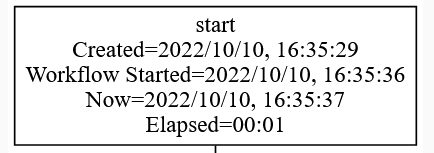
\includegraphics[width=0.7\columnwidth]{images/labelmaker-example.png}
\caption{An example node with labels}\label{fig:label-node}
\end{figure}

\begin{table}[htb]
\caption{List of possible labels for nodes on the graph}
\label{fig:labels-list}

{\footnotesize
\begin{tabular}{p{3.5cm}p{4cm}}
Name & Description \\
\hline
progress &  progress of job from 0-100 \\
now & current time \\
now.\verb|%Y%m%d,%H--%M--%S| &
   now in particular format (this can be used for other times as well) \\
created & time when workflow was created \\
t0.\verb|%Y%m%d,%H--%M--%S| &  workflow start time \\
t1.\verb|%Y%m%d,%H--%M--%S| & workflow end time \\
dt0.\verb|%Y%m%d,%H--%M--%S| & elapsed time since workflow began \\
dt1.\verb|%Y%m%d,%H--%M--%S| & total time of workflow once complete \\
tstart.\verb|%Y%m%d,%H--%M--%S| & job start time \\
tend.\verb|%Y%m%d,%H--%M--%S| & job end time \\
modified.\verb|%Y%m%d,%H--%M--%S| & job modified time \\
os. & operating system environment variable (like os.HOME) \\
cm. & cloudmesh variable that is read from \verb|cms set| \\
\end{tabular}
}
\end{table}



\subsection{Shapes and Styles}

As we use graphviz for rendering we have also added the ability to
change the shape and style for each nodes in the graph. The
available \href{https://graphviz.org/doc/info/shapes.html}{shapes}
and \href{https://graphviz.org/docs/attr-types/style/}{styles} are
listed in the Graphviz documentation \cite{www-graphviz}.

Figure \ref{fig:shape-style-yaml} is an example of a node in YAML
format that uses a box shape and an empty style. The empty style
defaults to \mintinline{bash}|filled|, which allows the node to change
color when the job status is changed.

\begin{figure}
    \begin{minted}[breaklines]{yaml}
    workflow:
      nodes:
        start:
          label: 'start\nCreated={created.%Y/%m/%d, %H--%M--%S}\nWorkflow Started={t0.}\nElapsed={dt0.}'
          kind: local
          user: grey
          host: local
          status: ready
          exec: 'echo hello'
          name: start
          shape: box
          style: ''
    \end{minted}
    \caption{Example of YAML config file that uses shape and style}
    \label{fig:shape-style-yaml}
\end{figure}



\subsection{Reporting Progress}\label{reporting-progress}

When running scripts/jobs inside a workflow, the scripts must leverage
some format of {\em cloudmesh.progress} to notify the user and the
backend client monitoring system. If progress is not reported, the
Workflow class cannot tell if the scripts are done.

The examples that are provided with cloudmesh-cc are already augmented
with {\em cloudmesh.progress}. Thus, if a user is running jobs through
cloudmesh cc workflows, they must integrate progress strings into the
log files that are monitored. This is available for shell and batch
scripts, Python and Jupyter.

For shell and Slurm scripts, the script must contain progress update
lines as follows:

\begin{minted}[breaklines]{bash}
echo "# cloudmesh status=running progress=1 pid=$$"
\end{minted}

at the beginning of the script, and

\begin{minted}[breaklines]{bash}
echo "# cloudmesh status=done progress=100 pid=$$"
\end{minted}

at the end of the script.

For Python scripts and Jupyter notebooks, the script it is easiiests
to use our build in progress method. and import it from the
cloudmesh.common module. The following example demonstrates its use:

\smallskip
\begin{minted}[breaklines]{python}
from cloudmesh.common.StopWatch import progress
from cloudmesh.common.Shell import Shell
filename = Shell.map_filename('./py_script.log').path
progress(progress=1, filename=filename)
# execute your analysis here ...
progress(progress=100, filename=filename)
\end{minted}
\smallskip

When recording progress, the progress should be ascending between 1
and 100. The last value must report 100 or the node will not be
completed and the Workflow gets stuck.  The output of the progress
will be written into a \verb|{workflowname}.log| file that will be
probed continiously by the client to report the progress to the user.

\subsection{Generating Progress Image as Graph}

The framework has a build in capability to export the progress of the
workflowin a DAQ.

Figure \ref{fig:workflow-process} shows
the execution and display graph of the workflow
over time.


In Figure \ref{fig:workflow-process} we depict a simple example
workflow to be executed where each task is executed sequentially. The
status of the execution can be displayed as table or as graph. In
Figure \ref{fig:workflow-process}, we showcase how the graph changes
its appearance over time while using no lable in the start and end
node and the label in the nodes for fetch-data, compute, and analyze:

\begin{minted}[breaklines]{bash}
label: "{name}\nprogress={progress}"
\end{minted}

\begin{figure}[htb]
\resizebox{1.0\columnwidth}{!}{
\begin{minipage}[b]{0.18\textwidth}
Definition and start \\
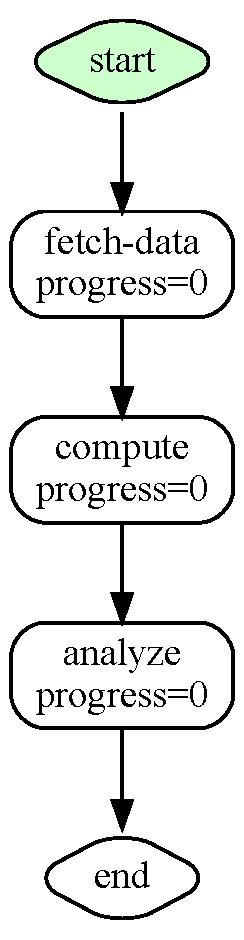
\includegraphics[height=9cm]{images/workflow-example-1.pdf}
\end{minipage} \ \
\begin{minipage}[b]{0.18\textwidth}
Running 1st task \\
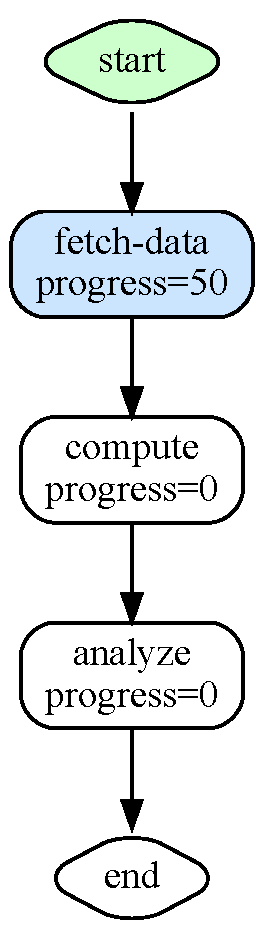
\includegraphics[height=9cm]{images/workflow-example-1.5.pdf} 
\end{minipage} \ \
\begin{minipage}[b]{0.18\textwidth}
Complete 1st task \\
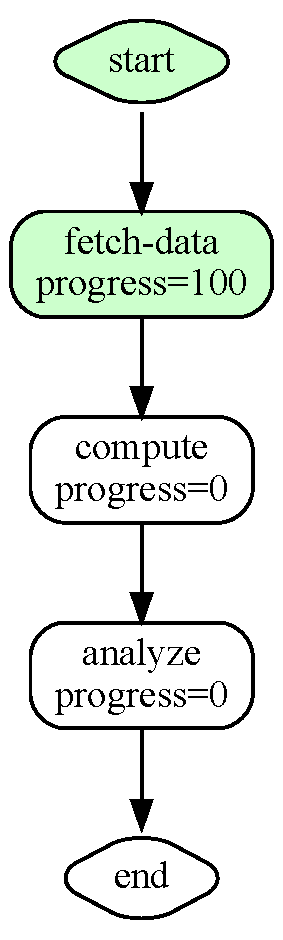
\includegraphics[height=9cm]{images/workflow-example-2.pdf}
\end{minipage} \ \
\begin{minipage}[b]{0.18\textwidth}
Complete 2nd task \\
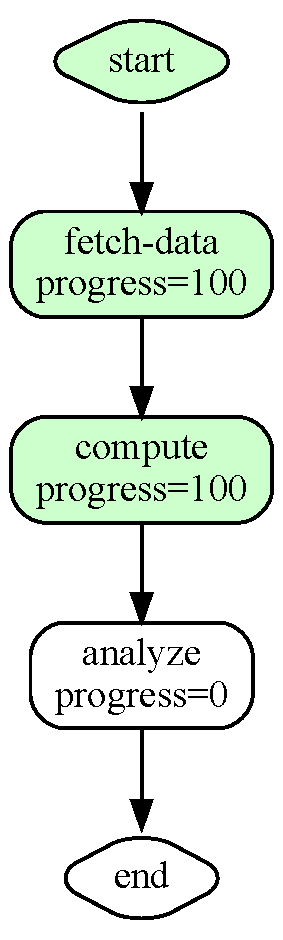
\includegraphics[height=9cm]{images/workflow-example-3.pdf}
\end{minipage} \ \
\begin{minipage}[b]{0.18\textwidth}
Complete workflow \\
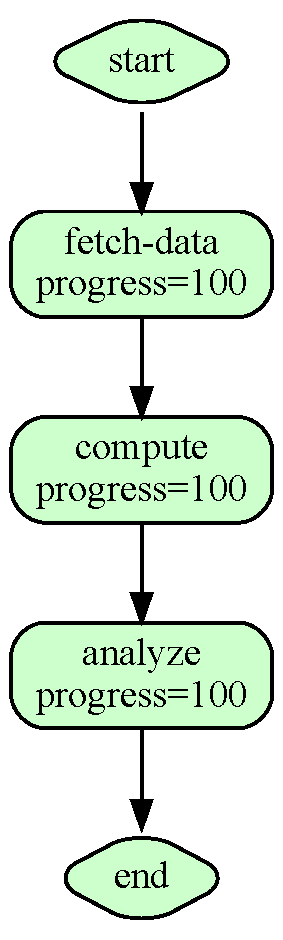
\includegraphics[height=9cm]{images/workflow-example-5.pdf}
\end{minipage} 
}
\caption{The gradual process of a simple workflow}\label{fig:workflow-process}
\end{figure}


